% ===========================================
% Data Processing
% Written by: Braidan Duffy
%
% Date: 06/22/2022
% Last Revision: 06/22/2022
% ============================================

\setchapterstyle{kao}
\chapter{Data Processing}
\setchapterpreamble[u]{\margintoc}
\labch{data_processing}
% \addcontentsline{toc}{chapter}{Data Processing} % Add the preface to the table of contents as a chapter

Data collected from sensors can sometimes be useful on their own, but often times, it is necessary to process it to gain a better understanding of what is occurring.
To that end, this chapter will be about how to process raw data into something more usable and some techniques that you can employ for your projects in the future.

    \section{Digital Filtering} \labsec{digital_filtering}
    One of the most fundamental data processing techniques is that of the digital filter.
    The idea behind these filters is to take in data samples and apply mathematical formulations on them to dampen undesirable signals within.

        \subsection{Kalman Filter} \labsec{kalman_filter}
        \subsubsection*{Introduction} The Kalman Filter is a recursive algorithm introduced in the 1960's as a method to track, estimate, and predict the state of a system and corresponding uncertainties.
        This filter integrates a dynamic (linear) model of the system, control inputs, measurements, and biases/uncertainties into a single algorithm.
        This effectively fuses together system inputs and responses and extrapolates what the system is currently doing and expected to do.
        One key advantage of this algorithm is that it only requires the guess of the previous state to estimate the current state. 
        This massively decreases the memory and processing costs as the history of inputs, measurements, and uncertainties does not need to be remembered or analyzed.
        However, it does have some limitations when the sensor data is noisy or the control inputs cannot be linearly mapped to the system state.
        Random errors in the sensor data may cause the filter to behave unpredictably and non-linearity prevents proper fusion entirely.\sidenote{Though this can be managed with an Extended Kalman Filter}

        This section will discuss the Kalman filter in a higher-order method.
        Many resources around with Internet can discuss the in-depth mathematics governing this filter and you are free to browse them at your leisure. 
        For this guide, my primary concern is to get you acquainted with the Kalman filter and its broader practical applications.
        
        \subsubsection*{Background} This section assumes that you do not have a lot of background knowledge on basic statistics and terminology.
        It is important to understand here that mean and expected value are not the same thing.
        In many college lab courses, measurements are taken multiple times and averaged together to find the mean value (often denoted as $\mu$).
        This is assumed to be the absolute correct value with zero uncertainty.
        However, this is never the case in the real world as all measurements have uncertainty in some fashion.
        When the average measurement value is taken \textit{with} uncertainties factored in, this becomes the expected value ($E$) and used to guess what the real (correct) value of the measured variable is.

        So, how can quantify the uncertainties within the expected value? First, we need to know what the measurement variance is.
        This value is a description of how far the measured data is from the mean and is defined in Equation \ref{eq:variance}. \sidenote{For large datasets, variance is normalized by $\frac{1}{N-1}$}

        \marginnote{The standard deviation of the dataset $\sigma$ decribes the probabalistic distance a measurement can have from the mean and is defined by:
        \begin{equation*}
            \sigma = \sqrt{\sigma^2}
        \end{equation*}
        }
        
        \begin{gather} \labeq{variance}
            \sigma^2 = \frac{1}{N} \sum_{n=1}^{N} (x_n - \mu)^2 \\ 
            \begin{aligned}
                \text{where } &\sigma^2 \text{ is the variance} \\
                &N \text{ is the total number of samples} \\
                &x_n \text{ is the n-th sample} \\
                &\mu \text{ is the running average}
            \end{aligned} \notag
        \end{gather}

        \begin{kaobox}[frametitle=Aside: Normal Distribution]
            Normal distribution of data is the archetypical bell curve.
            It is also referred to Gaussian distribution and is defined by:
            \begin{equation*}
                f(x, \mu, \sigma^2) = \frac{1}{2\pi\sigma^2} \exp{\frac{-(x-\mu)^2}{2\sigma^2}}
            \end{equation*}
            This function creates a Gaussian curve which is the Probability Density Function (PDF) for a normal distribution.
            Normally, measurements errors are Gaussian-distributed and the Kalman filter assumes this is always the case.
            Different error distributions will drastically increase the uncertainties within the filter and may negate it entirely.
        \end{kaobox}
        
        \begin{marginfigure}[-2in]
            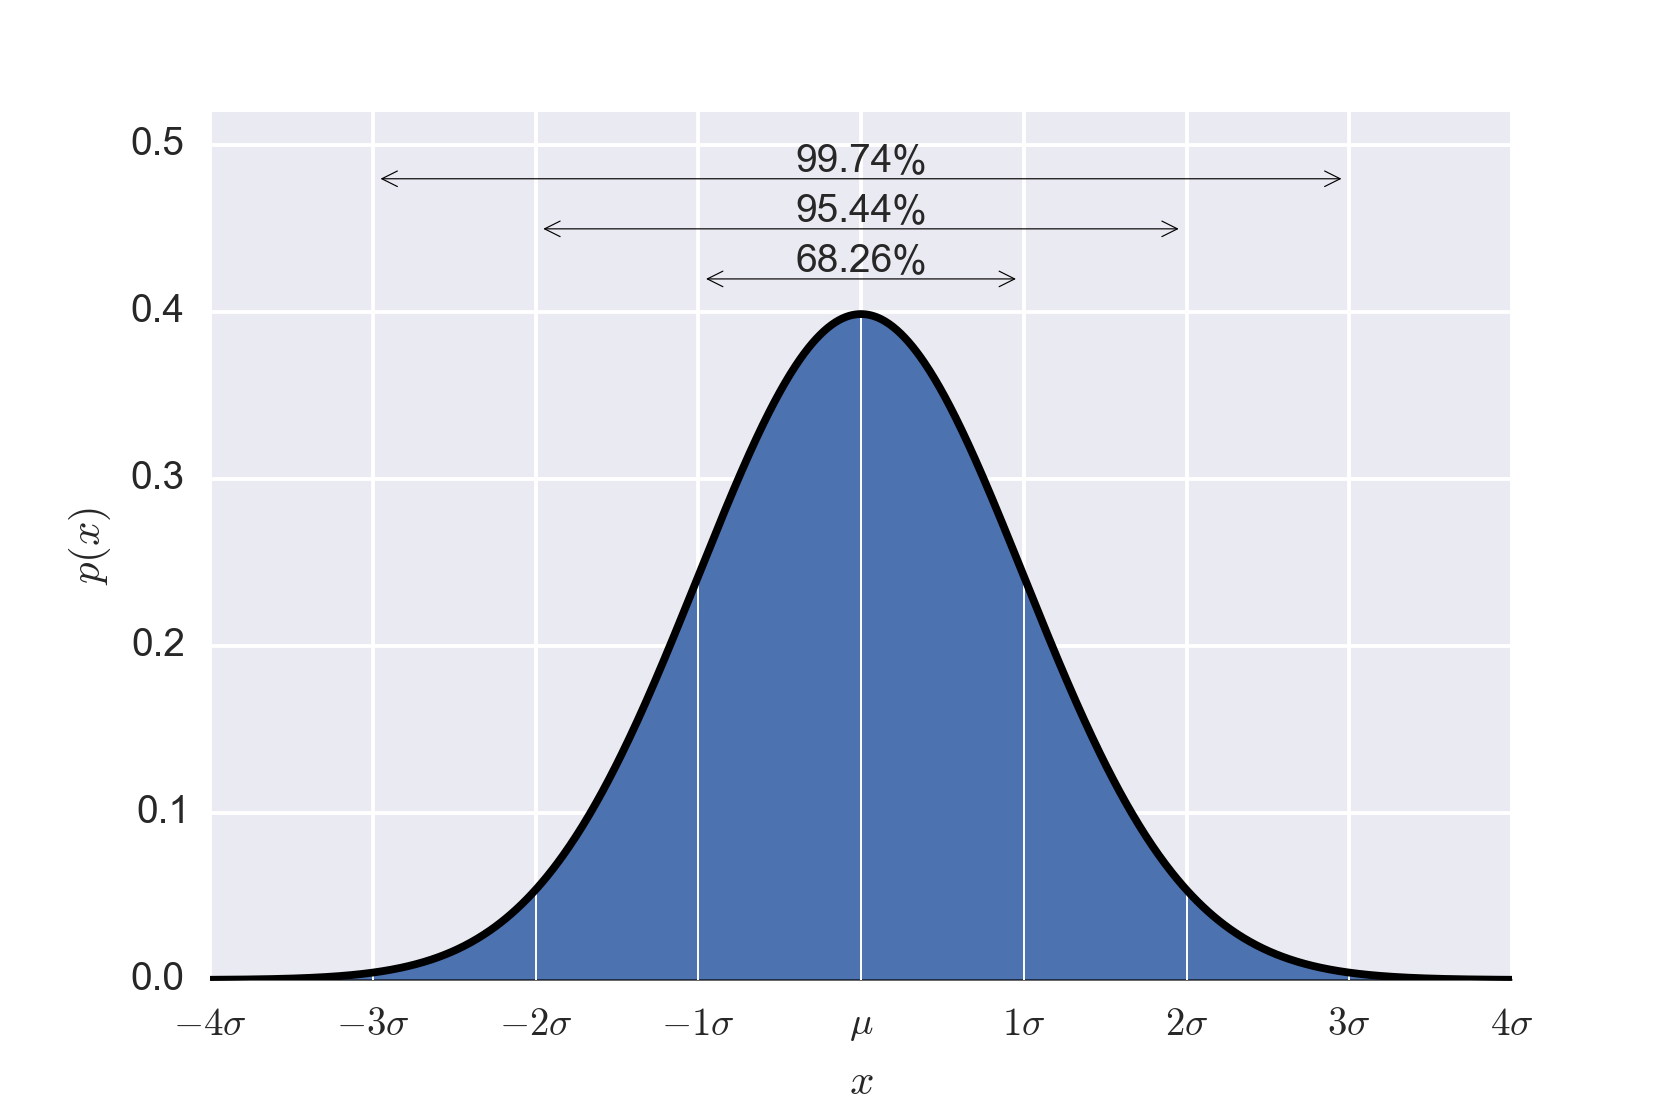
\includegraphics[]{data_processing/gaussian_distribution.png}
            \caption[Aside: Gaussian Distribution]{A graph of a Gaussian distribution with the 1st standard deviations shown.
            Retrieved from \href{https://accadandkoka.com/blog/how-normal-is-the-normal-distribution/}{The Akkad and Koda Report}}
            \labfig{aside_gaussian_dist}
        \end{marginfigure}

        Estimates are the algorithm's guessed value at the unknown system state.
        Here, accuracy quantifies how close the estimate is to the true value whereas precision quantifies the variability of the estimates with respect to uncertainty.
        High precision estimates have a low variance (uncertainty) in measurements.
        Low accuracy estimates display a bias that are systemic errors in measurement.
        Variance is determined by random measurement error and can be reduced by averaging or smoothing the measurements.

        \begin{figure*}[h!]
            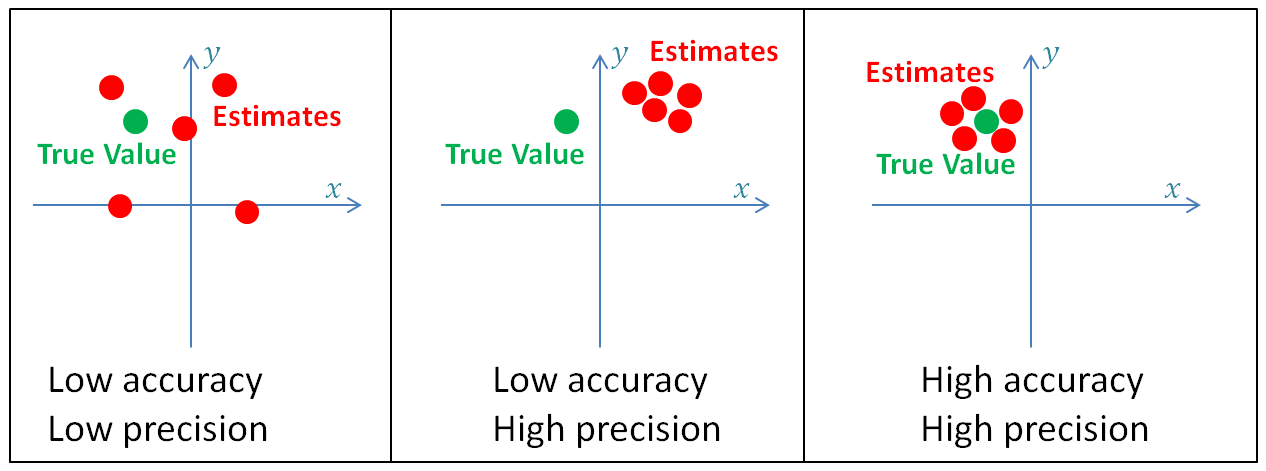
\includegraphics[]{data_processing/AccuracyAndPrecision.png}
            \caption[Accuracy and Precision]{Different plots demonstrating the difference between accuracy and precision.
            Retrieved from \href{https://www.kalmanfilter.net/img/BB1/AccuracyAndPrecision.png}{KalmanFilter.net}}
            \labfig{accuracy_precision}
        \end{figure*}

        \subsubsection*{The $\alpha$ Filter} At any sample, $N$, a value $\hat{x}_{N,N}$ can be estimated using:
        
        \begin{gather*} \labeq{sample_estimate}
            \hat{x}_{n,n} = \frac{1}{N} \sum_{n=1}^{N} (z_n) \\
            \begin{aligned}
                \text{where } &\hat{x}_{n,n} \text{is the estimate of the true value at sample $n$} \\
                &N \text{ is the total number of samples taken} \\
                &n \text{ is the current sample number} \\
                &z \text{ is the current measurement} \\
            \end{aligned} \notag
        \end{gather*}

        Since the estimate accuracy will improve with the number of measurements, we need to remember all the historical measurements.
        However, storing, accessing, and operating on discrete measurements exponentially increases in difficulty and computational power as more measurements are taken.
        Therefore, we can store the previous measurements in a state variable and add a small adjustment that is proportional to the newest measurement.
        This preserves the accuracy of storing many discrete data points and the computing and storage resources required to operate on data added to the set.

        This algorithm is called the \textit{State Update Equation} and is one of the five Kalman equations. 
        It is defined by:

        \begin{gather} \labeq{state_update_eq}
            \hat{x}_{n,n} = \hat{x}_{n,n-1} + \alpha_n(z_n - \hat{x}_{n,n-1}) \\
            \begin{aligned}
                \text{where } &\hat{x}_{n,n} \text{is the estimate of the true value at sample $n$} \\
                &\hat{x}_{n,n-1} \text{ is the estimate of the previous true value} \\
                &n \text{ is the current sample number} \\
                &\alpha_n \text{ is a correction gain} \\
                &z \text{ is the current measurement} \\
            \end{aligned} \notag
        \end{gather}

        \marginnote[-1.5in]{The correction gain, $\alpha_n$ is unique to every example and can change with every sample.
        It is also called the Kalman gain, denoted by $K_n$}

        \marginnote[-0.75in]{The term $(z_n - \hat{x}_{n,n-1})$ is the measurement residual or "innovation"; this contains the new information.}

        This algorithm uses zero-indexing, so the initial or starting guess will be $n=0$.
        This value can be determined by reasoning or physical constraints of the system.
        The filter will always require an initial guess to kickstart the algorithm.
        A flow chart describing the algorithm's process is below.

        \hl{INSERT ALPHA FILTER FLOW CHART HERE!}
        
        \pagelayout{wide} % No margins

        \begin{example} Let's say that we are programming a scale to estimate the weight of an ROV placed atop it.
        For the sake of example, we know that the ROV weighs exactly 10 kilograms and we want to quantify the uncertainty of our scale. 
        \paragraph{Iteration 0}
        \begin{gather*}
            \begin{aligned} 
                0:& \text{ We can guess that the initial weight of the ROV is 10-kg: } \hat{x}_{0,0} = 10 \text{ kg} \\
                3:& \text{ Since the weight should not change, our prediction for the next measurement is: } \hat{x}_{1,0} = \hat{x}_{0,0} = 10 \text{ kg} \\
            \end{aligned}
        \end{gather*}
        
        \paragraph{Iteration 1}
        \begin{gather*}
            \begin{aligned} 
                1:& \text{ We make a measurement on the scale: } z_1 = 10.3 \text{ kg} \\
                2\text{a}:& \text{ We calculate the correction gain: } \alpha_1 = \frac{1}{N} = \frac{1}{1} = 1 \\
                2\text{b}:& \text{ We can then estimate the current state: } \hat{x}_{1,1} = \hat{x}_{1,0} + \alpha_1(z_1 - \hat{x}_{1,0}) = 10 + 1(10.3 - 10) = 10.3 \text{ kg} \\
                3:& \text{ Since the weight should not change: } \hat{x}_{2,1} = \hat{x}_{1,1} = 10.3 \text{ kg} \\
            \end{aligned}
        \end{gather*}

        \paragraph{Iteration 2}
        \begin{gather*}
            \begin{aligned} 
                1:& \text{ We make a measurement on the scale: } z_2 = 9.9 \text{ kg} \\
                2\text{a}:& \text{ We calculate the correction gain: } \alpha_2 = \frac{1}{N} = \frac{1}{2} = 0.5 \\
                2\text{b}:& \text{ We can then estimate the current state: } \hat{x}_{2,2} = \hat{x}_{2,1} + \alpha_2(z_2 - \hat{x}_{2,1}) = 10.3 + 0.5(9.9 - 10.3) = 10.1 \text{ kg} \\
                3:& \text{ Since the weight should not change: } \hat{x}_{3,2} = \hat{x}_{2,2} = 10.1 \text{ kg} \\
            \end{aligned}
        \end{gather*}

        \end{example}

        \pagelayout{margins} % Replace margins
        
